\chapter{理论与相关工作}
\label{chap:theory}
在这一章,我们将会对涉及到的理论,算法原理与相关工作进行介绍。
\section{博弈树}
% 博弈论就是研究博弈行为中斗争各方是否存在着最合理的行为方案,以及如何找到这个合理的行为方案的数学理论和方法~\cite{gt}。
博弈树(game tree)用来表达由博弈行为所产生的各种可能性以及后续衍生情况。博弈树从起始节点出发,向下延展出若干层的子节点直到当前博弈结束~\cite{gt}。
下一层的子节点是基于其父节点博弈行为所导致的可能性结果。博弈树的叶节点代表博弈结束的可能状态,例如井字游戏(Tic-Tac-Toe)会有~26830~个叶节点~\cite{NAU1982257,allis1994searching}。


博弈树在人工智能应用领域占有重要地位,在博弈游戏中选择最佳动作的一种常见方法便是使用某种树搜索算法,结合类似于极小化极大算法的规则来修剪树,从而搜索整个博弈树。
例如在井字游戏中计算机可以很快速地找到最佳解并做出决策,但是对于象棋、围棋这一类状态空间复杂的大型博弈游戏,受限于计算机性能遍历整个博弈树往往不太现实,会花费巨量的时间,因此对这类游戏往往会选择搜索部分博弈树(partial game tree)。
较为常见的做法是限制博弈树的层数深度,并剪掉不佳的走法节点(例如将军),在这种情况下,搜索的层数更多,能走出较佳走法的机会也越高~\cite{coin12162}。

\subsection{极小化极大算法}
极小化极大算法(Minimax)是人工智能领域常见的搜索算法,是一种最小化对手最大收益的算法,常用于棋类等游戏。
该算法是一种零和算法,即一方要在合法的选项中选择最大化其收益的选择,而另一方则选择令对手优势最小化的方法~\cite{ctt1r2gkx}。

\begin{figure}[htb]
    \centering
    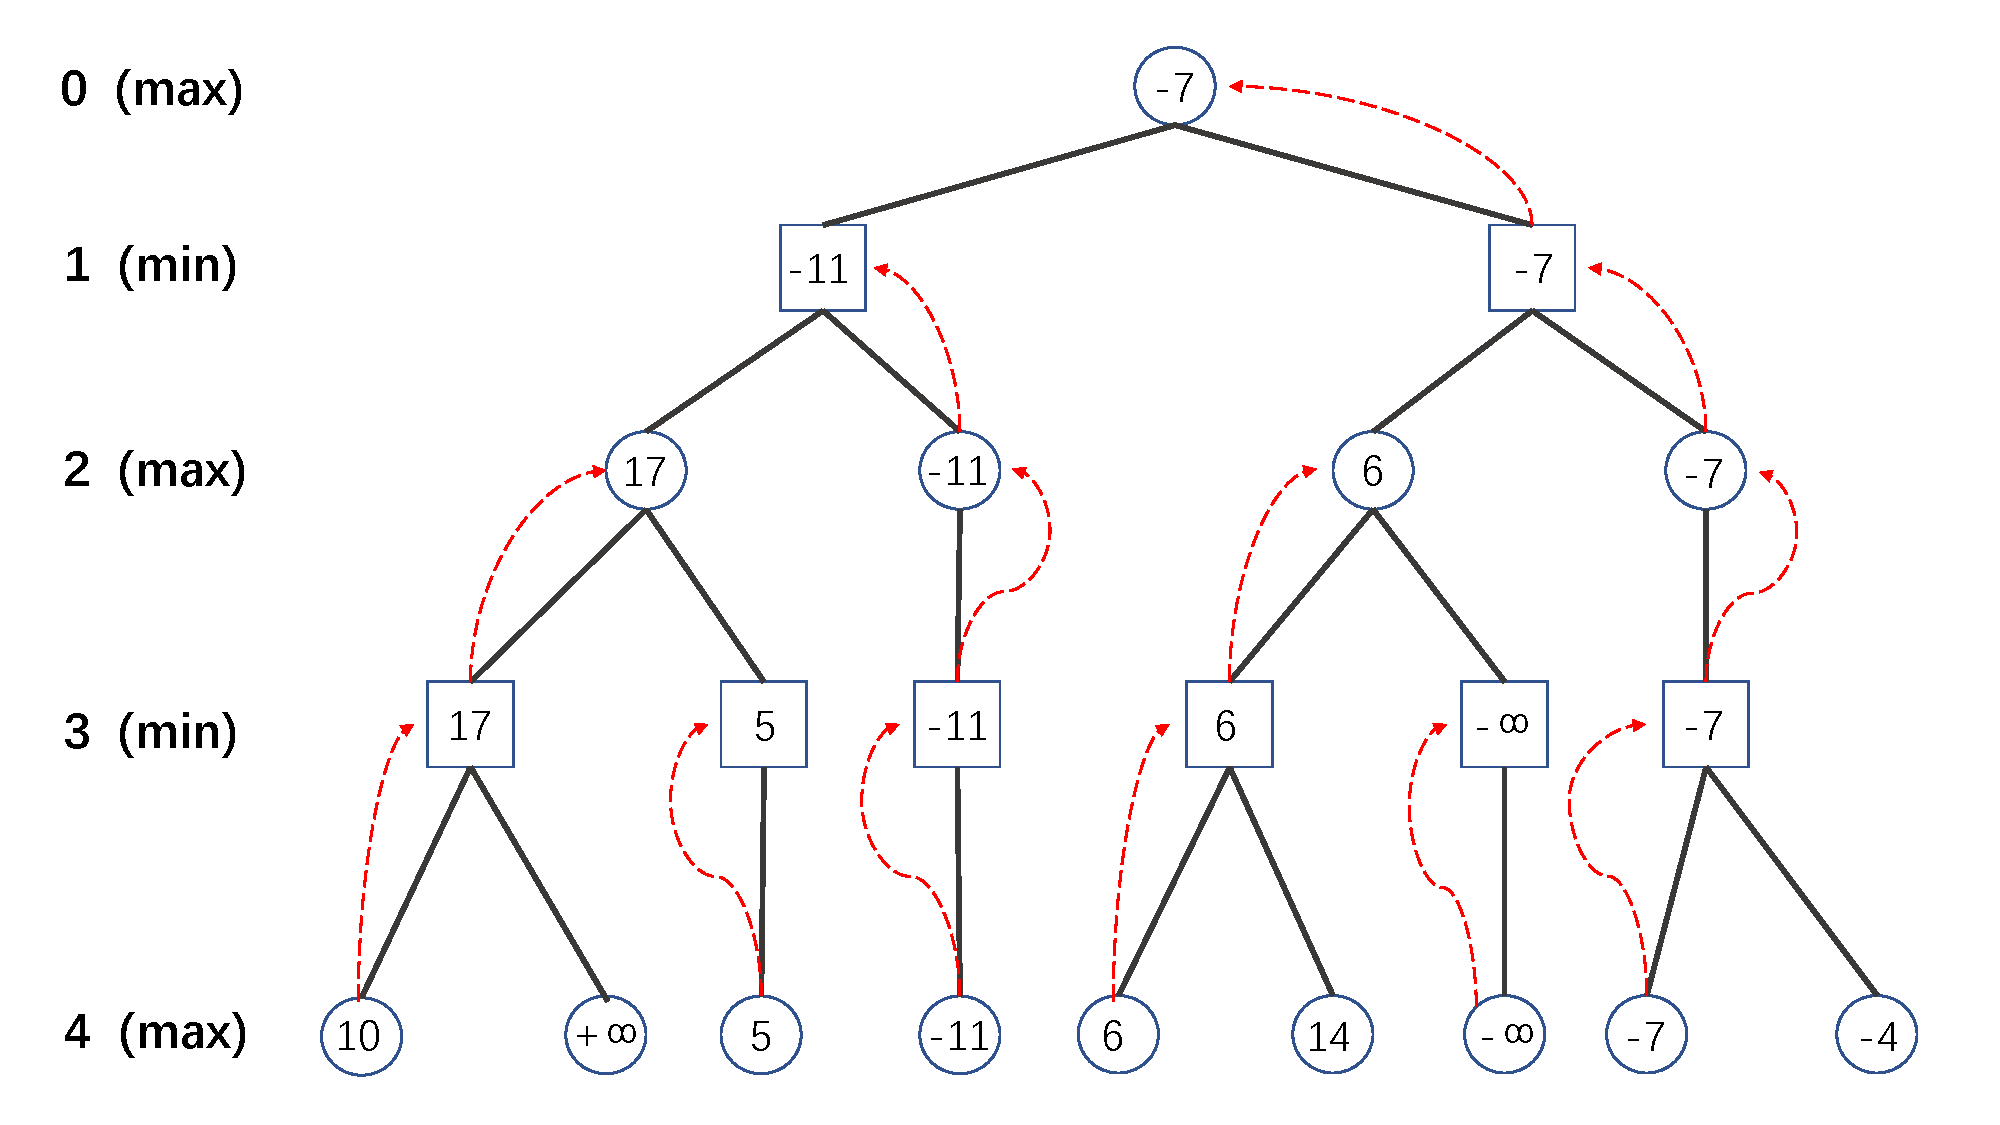
\includegraphics[width=1\textwidth]{Minimax.pdf}
    \caption[minimax]{%
      极小化极大算法搜索树例子~\cite{wikiMinimax}%
      }
    \label{fig:minimax}
  \end{figure}

如图~\ref{fig:minimax}~所示,假设圆形代表当前选手,方形代表对手。当前选手需要将自己所得分数最大化,而对手则需要反其道行之。
考虑第三层(Min层)对手在最左侧节点的决策,当前选手在第四层有得分为10或正无穷的行动选择,对手想要做出一个最小化我方收益的选择,即选择得分为10的行动。其余同理。
\subsection{alpha-beta 剪枝}
在上一个小节中我们介绍了经典的极小化极大算法,对于一个具有复杂状态空间的游戏(象棋或围棋)来说,极小化极大算法需要非常多层才能够完成,
其在遍历搜索树时具有指数级复杂度。在这种情况下,使用经典的极小化极大算法进行树搜索是不现实的。
因此我们就需要采取某种方式减少运算量,而剪掉一些不需要搜索的分支是一种直接的思路。

最经典的剪枝算法为~alpha-beta~剪枝,剪枝的含义为剪掉不需要搜索的节点。其中$\beta$值为可行解的最小上界(Min层通向根节点的路径上最好的选择),$\alpha$值为可行策略(解)的最大下界(Max层通向root的路径上最好的选择)。
其在生成博弈树的同时计算评估各节点的$\alpha$值与$\beta$值, 并且根据其值范围, 停止搜索无用节点,以提高运算速度。该算法与极小化极大算法在同一局游戏中会得出相同的结果,因为剪去了不影响决定的节点与路线分支使得搜索速度更快~\cite{russell2010artificial}。
剪枝过程遵循$\alpha \le N \le \beta$,N为当前节点评估值。即:(1)当一个 Min 节点的 $\beta$值小于等于任何一个父节点的$\alpha$值时 ,剪掉该节点的所有子节点;(2)当一个 Max 节点的 $\alpha$值大于等于任何一个父节点的$\beta$值时 ,剪掉该节点的所有子节点~\cite{russell2010artificial}。
我们用以下Minimax树(图~\ref{fig:abp})作为例子,方块为Max节点,圆形为Min节点~\cite{russell2010artificial}。
\begin{figure}[htb]
    \centering
    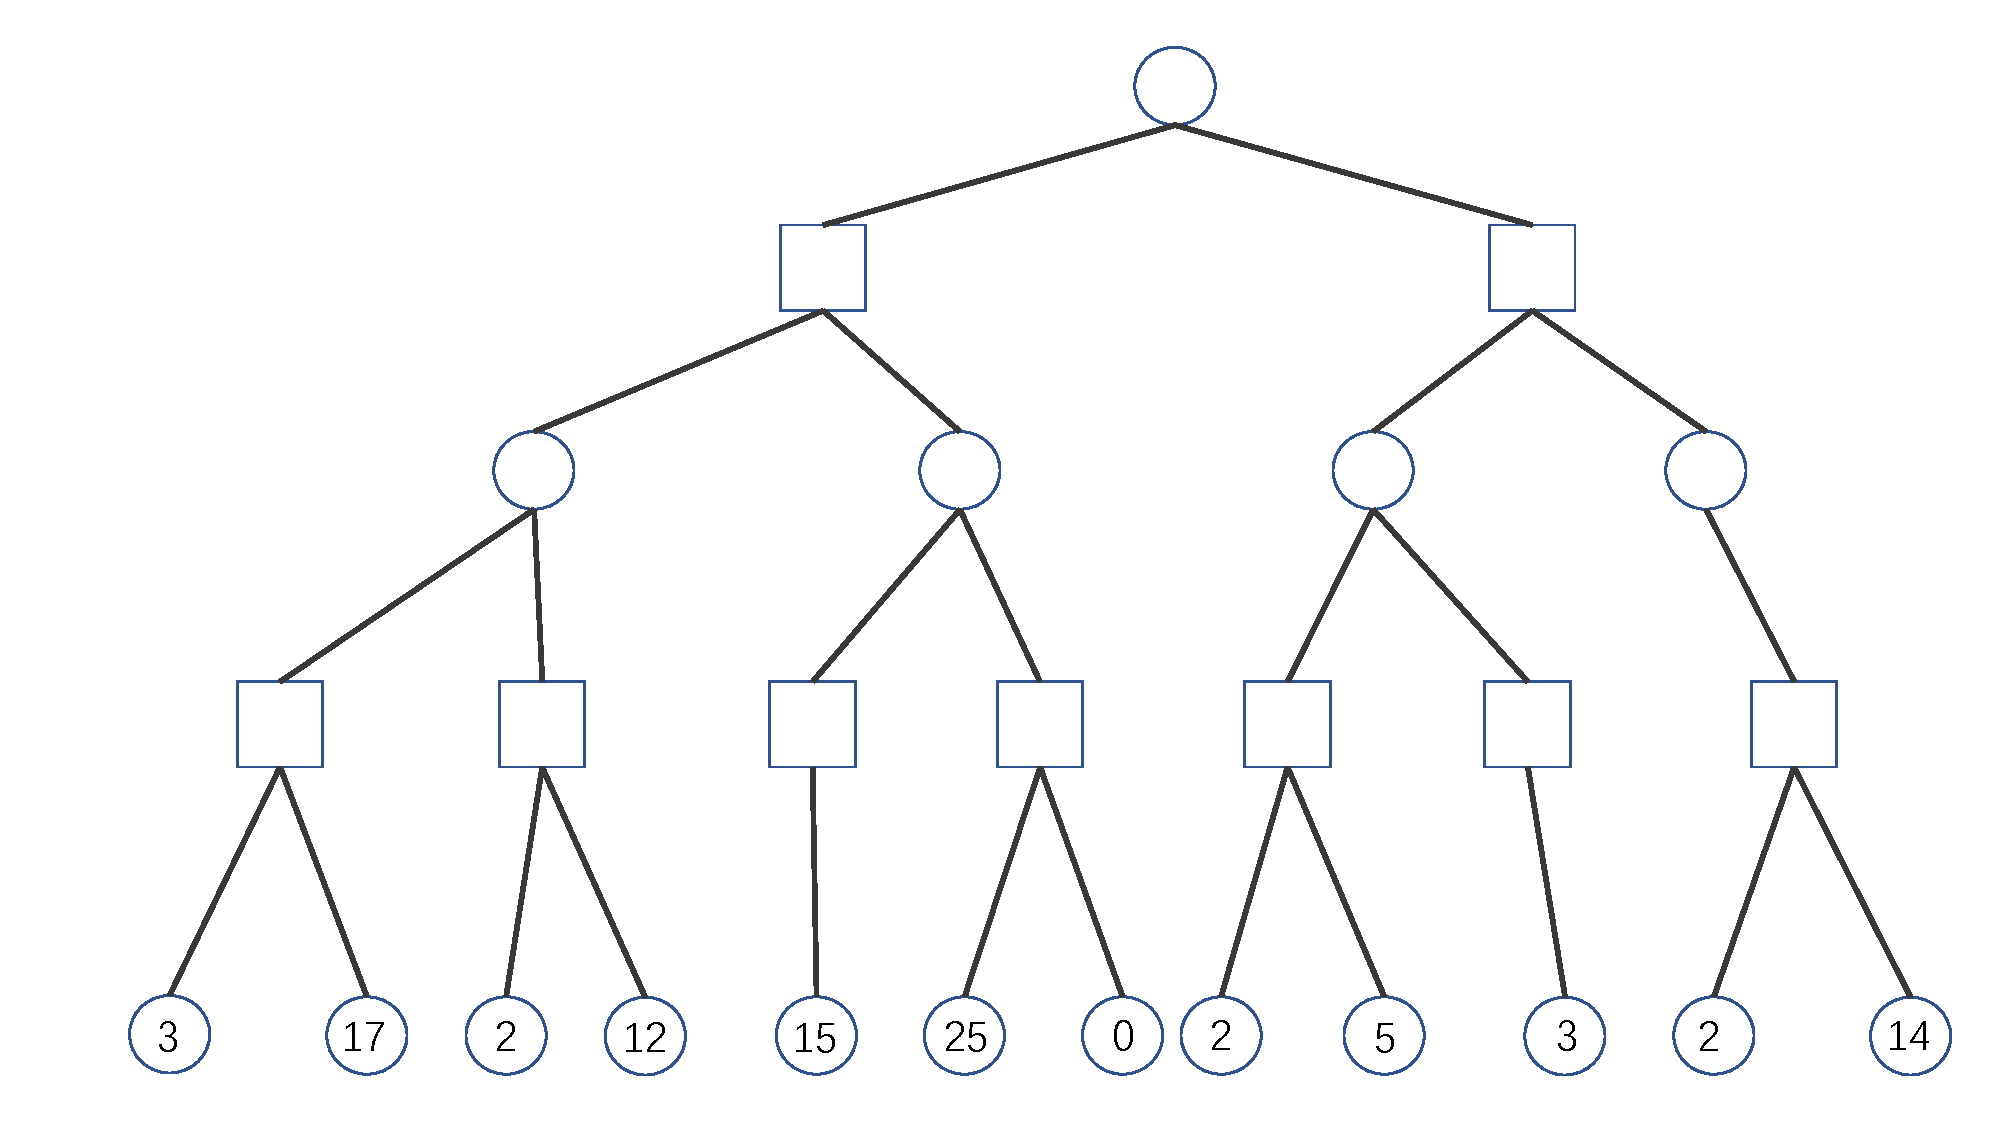
\includegraphics[width=0.9\textwidth]{abp1.pdf}
    \caption[abp]{%
    alpha-beta剪枝初始状态~\cite{russell2010artificial}%
      }
    \label{fig:abp}
  \end{figure}

其剪枝过程如图~\ref{fig:abp2}~所示。从左节点开始,

(1)对左边第一个子节点进行评估并获得值为5。将此节点值传给其父Min节点。该父节点的Minimax值必须$\le 5$,所以我们将该Min节点$\beta$值更改为5;

(2)接下来在深度为4层处遍历下一个子节点,并向父Min节点返回值11;

(3)父节点为Min节点,并且11大于5,忽略返回11的子节点。 此Min节点的所有子节点已评估完成,将$\beta$值返回到父Max节点。 Max节点的值将$\ge 5$,此时将其$\alpha$值更改为5:

(4)遍历该Max节点的其他Min子节点,并将当前的评估区间值传递给子节点;

(5)搜索新Min子节点的子节点,第一个值为1,传递给其父节点;

(6)父节点的值将$\le 1$,将其$\beta$值改为1;我们发现在此节点上找到解决方案路径的唯一方法是找到一个值大于5且小于1的子节点,然而该情况不可能出现。我们停止评估其他子节点,因为不论何值都不会让父Max节点选择比5更差的结果,然后我们返回$\beta$值(也就是1)作为该节点的值。
回到父Max节点,其$\alpha$值已经是5,比1更具限制性,因此不要更改它。我们已经看到了此Max节点的所有子节点,因此可以将其值设置为最终的$\alpha$值即为5。

\begin{figure}[htb]
    \centering
    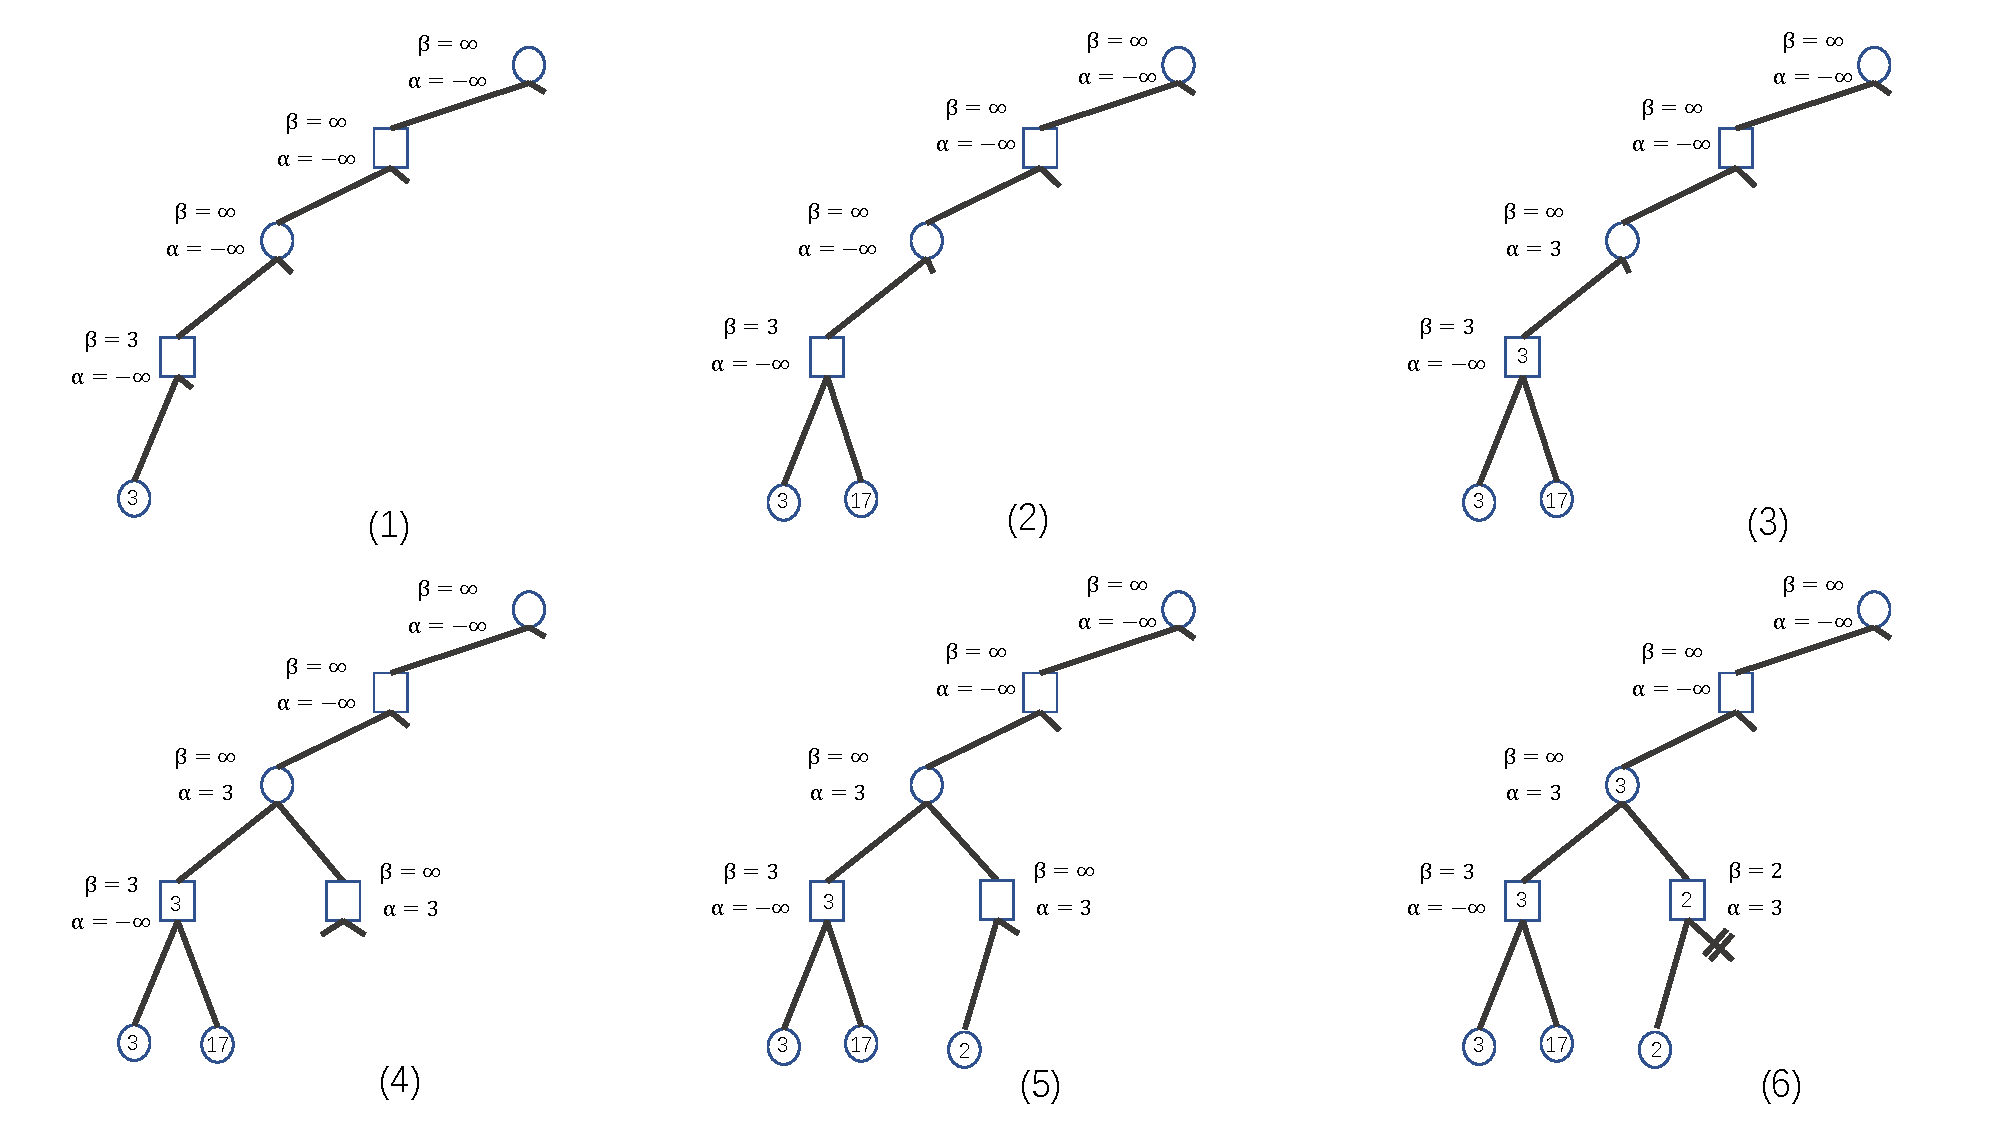
\includegraphics[width=1\textwidth]{abp2.pdf}
    \caption[abp2]{%
    alpha-beta剪枝过程演示,按顺序步骤从(1)到(6)~\cite{russell2010artificial}%
      }
    \label{fig:abp2}
  \end{figure}
\newpage
在极小化极大算法上,alpha-beta~剪枝做出了改进,通过减少搜索树的分支,提高搜索效率。
若节点搜索顺序达到最优化或近似最优化(将最佳选择排在各节点首位),则同样时间内搜索深度可达极小化极大算法的两倍多~\cite{KNUTH1975293abp}。但是对于较复杂的棋类游戏,若对每一步棋有落子时间限制,alpha-beta~剪枝的搜索深度依然受到较大限制,在实际应用中往往采取3--4层,也有可能导致只能获得局部最优解。
除此之外,对手玩家一定会选择使我方结果最差的思路的先验假设,在真实情况下并不正确,因为无法确定对方的博弈策略是否和自己一致。如果对方做的策略不是最优,那么我方所作出策略是最优的假设也将不成立。

\subsection{蒙特卡洛树搜索}
蒙特卡洛树搜索(Monte Carlo tree search,简写为~MCTS)是一种启发式搜索算法,广泛应用于博弈树搜索~\cite{10.1007/978-3-540-75538-8_7}。顾名思义,其设计思路是基于概率的:多次模拟游戏过程,并尝试根据模拟结果的胜负率预测最好的动作选择。
这也与人类下棋时的思维模式符合:根据感觉在大脑里思考出了若干种最有可能的落子选择,然后再思考假设落子后对手最可能的对应措施,如此反复进行选出最佳结果。

蒙特卡洛树搜索的每个循环包括四个步骤~\cite{RePEc:wsi:nmncxx:v:04:y:2008:i:03:n:s1793005708001094},如图~\ref{fig:mcts}:

(1) 选择(Selection):从根节点开始,采取某些算法对各节点打分如上限置信区间(Upper Confidence Bound,简写为~UCT)~\cite{10.1007/11871842_29},不停选择子节点直到遇到叶子节点;

(2) 扩展(Expansion):新增可能的子节点并选取一个作为下一轮中的根节点;

(3) 模拟(Simulation):从选定的节点开始,随机选择动作进行游戏;

(4) 回溯(Backpropagation):使用模拟步骤的结果,更新已探索路线上节点的属性值。

谷歌公司的AlphaGo/Zero体系中都使用了~MCTS~的架构并对其策略进行了改进与优化。

\begin{figure}[htb]
    \centering
    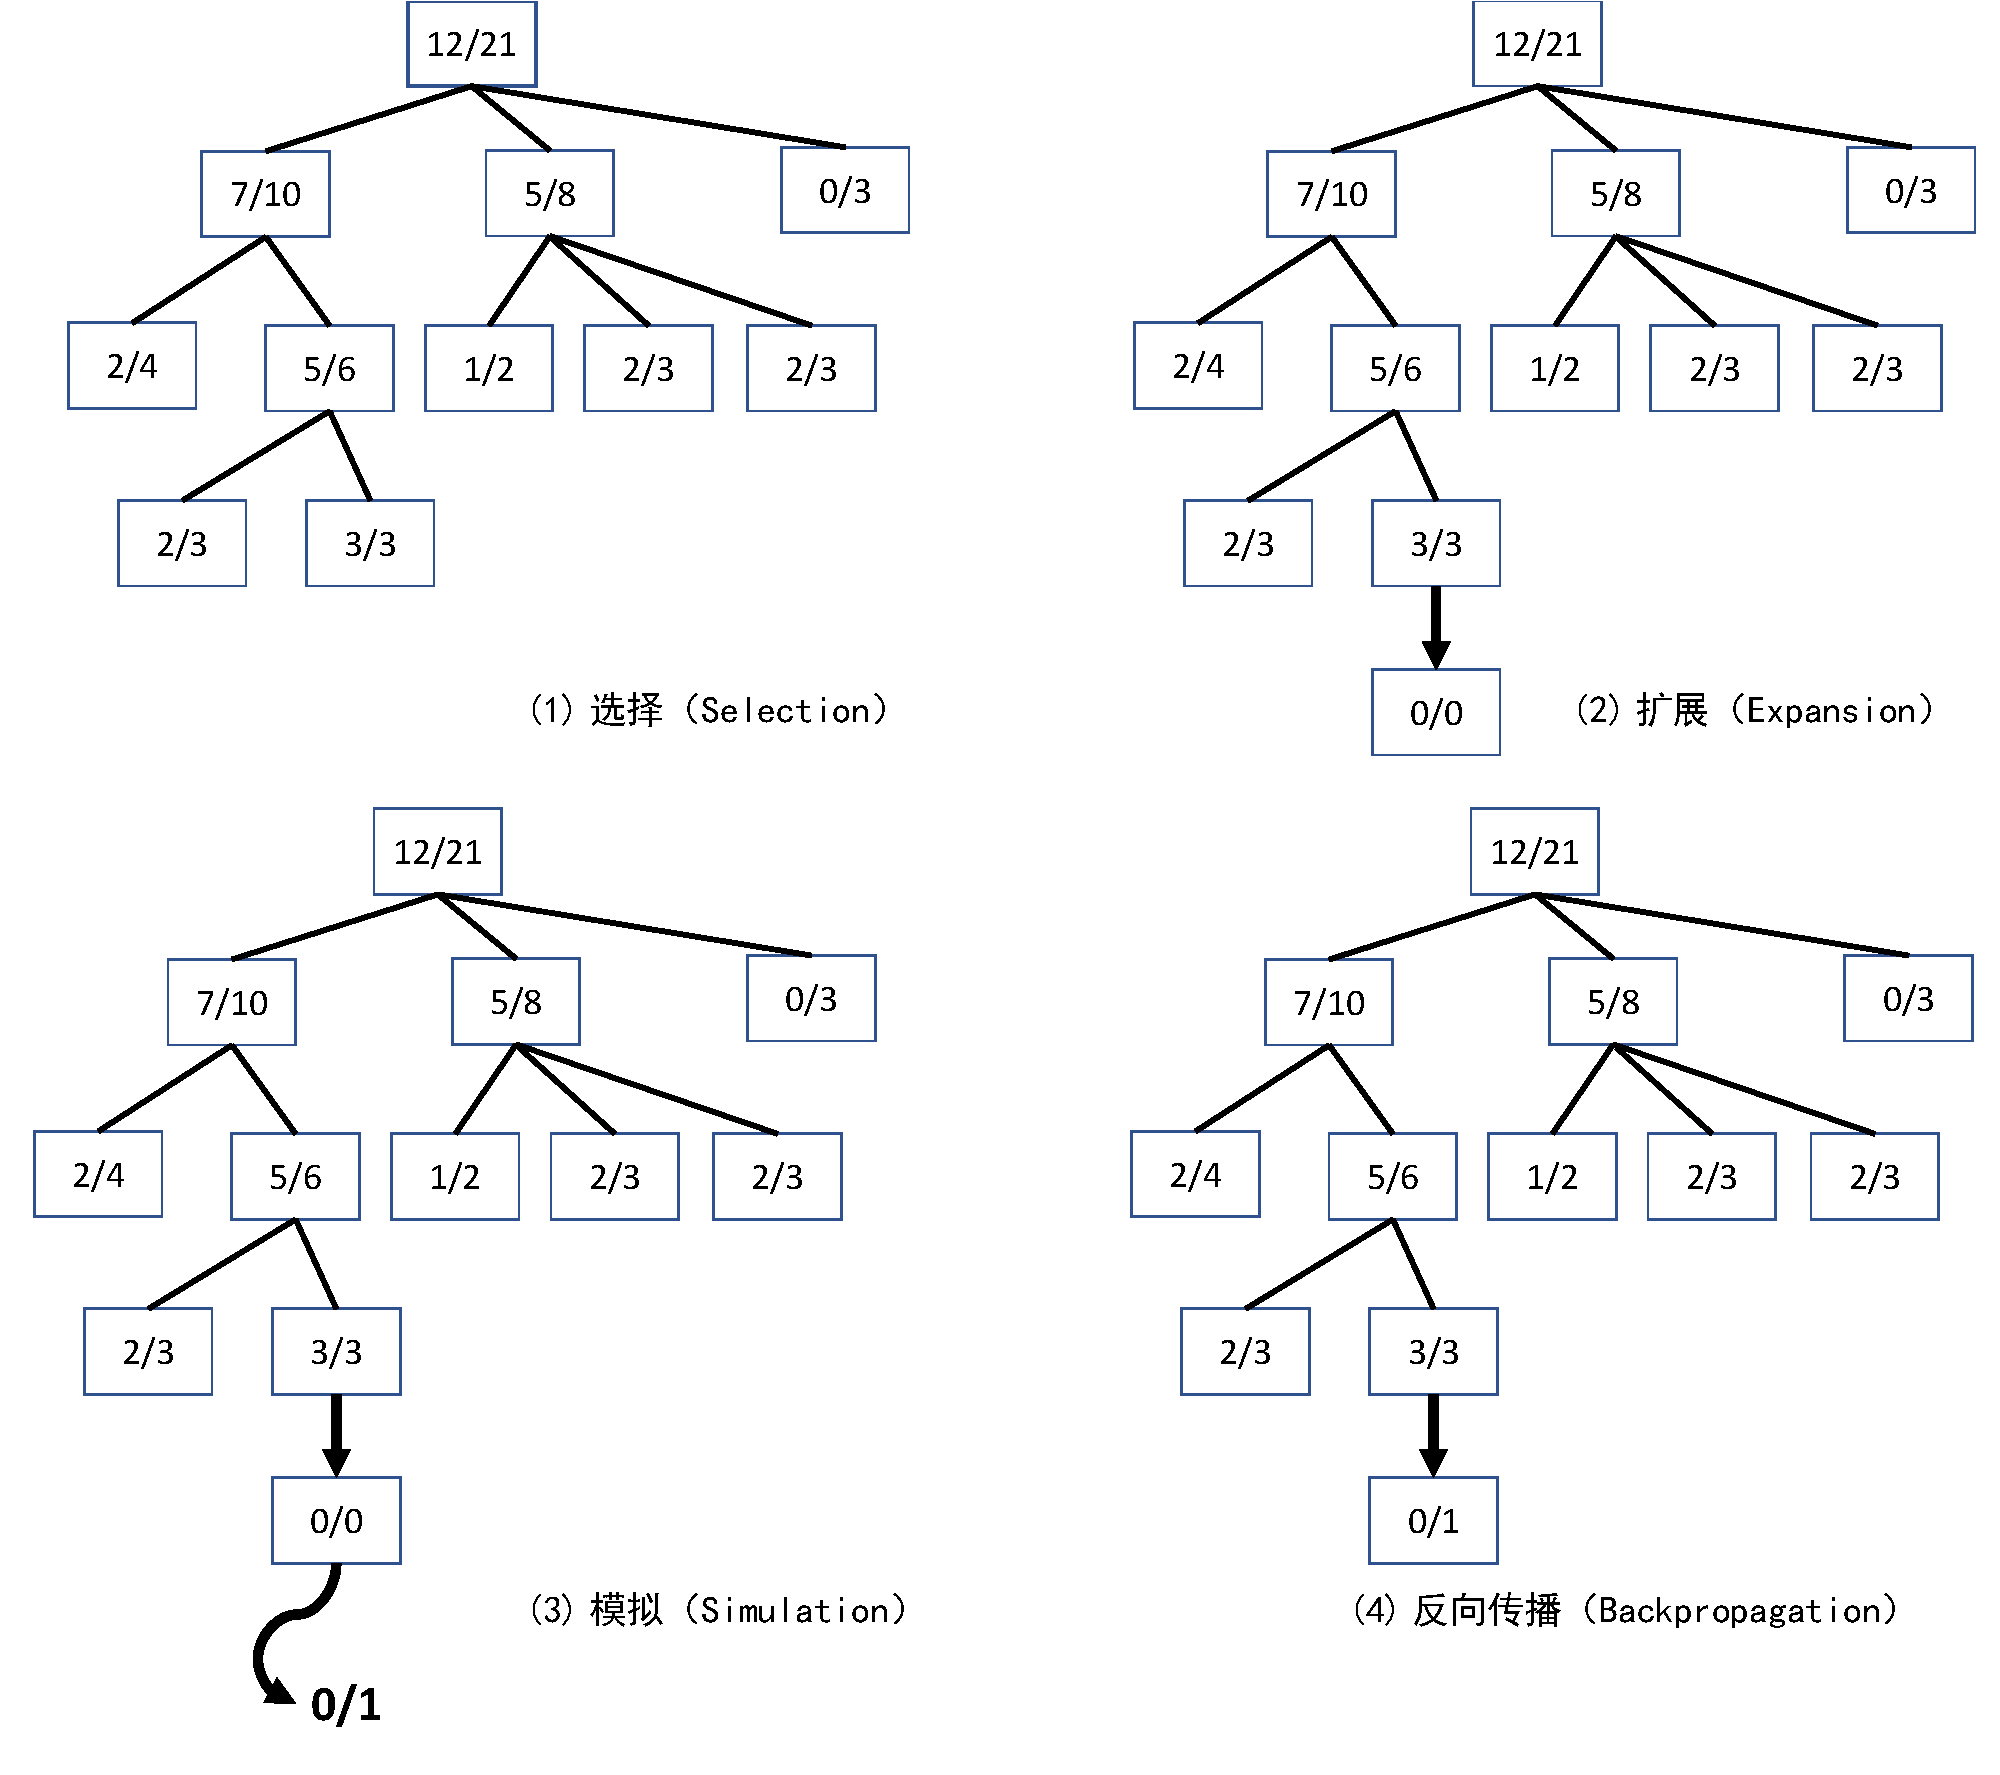
\includegraphics[width=0.9\textwidth]{mctswiki.pdf}
    \caption[mcts]{%
    蒙特卡洛树搜索的步骤,圆圈内的数字代表胜利数量/游戏数量~\cite{RePEc:wsi:nmncxx:v:04:y:2008:i:03:n:s1793005708001094}%
      }
    \label{fig:mcts}
\end{figure}

\subsubsection{选择子节点的方式}
在蒙特卡洛树搜索中,可以将节点分为3类:

\begin{itemize}
    \item [(1)] 
    未探索的节点:还没有评估过当前局势;
    \item [(2)]
    部分展开的节点:被评估过但未完全遍历子节点,可以继续扩展;
    \item [(3)]
    完全展开的节点:子节点已遍历。
\end{itemize}

搜索开始时,所有子节点都处于未被探索的状态,任意选择其中一个开始蒙特卡洛树搜索的模拟过程。当模拟结束后,其结果会回溯至当前博弈树的根节点。进行模拟的节点被标注为已探索。
回溯模拟结果的目的是更新相关路径上所有节点 $v$ 的奖励 $Q(v)$ 以及探索次数 $N(v)$。在实践中,$Q(v)$是该节点胜利的次数,$N(v)$是该节点模拟的次数。胜利次数多的节点是较好的可利用候选节点,从这类节点继续扩展可能可以维持胜率。
而模拟次数少意味着该节点在蒙特卡洛树搜索过程中探索次数少,具有尚未被发现的价值。
利用这两个节点属性构建树的置信上限(UCT)~\cite{10.1007/11871842_29}在被访问节点中选择下一个要遍历的节点:
\begin{equation*}
    \textbf{UCT}(v_{i},v) = \frac{Q(v_{i})}{N(v_{i})} + c\sqrt{\frac{\log(N(v))}{N(v_{i})}},
\end{equation*}
上式中$c$为一个常数,用来平衡高胜率(加号前面)与低访问次数(加号后面),$v_{i}$为$v$的子节点。
UCT值最大的节点就是蒙特卡洛树搜索遍历过程中选择的节点:每次选择己方 UCT 值最大的某个节点,向下搜索,直到找到一个部分展开的节点,该节点一定有未访问的子节点,随机选择某个子节点进行扩展。
扩展会为刚刚选择的节点加上一个统计信息为$(Q(v)=0,N(v)=0)$的节点,然后进入下一步模拟。
在我们后续使用~AlphaZero~架构构建超级皇后~AI~时,模拟的步骤可以直接使用神经网络进行评估~\cite{Silver1140,Silver2017,Silver2016}。

\section{卷积神经网络模型}
卷积神经网络(Convolutional Neural Network,简写为CNN)是一个超级大的话题,我们不打算在此进行过多阐述,仅进行少部分与棋类游戏AI相关的概念介绍,为后面方法设计部分打下理论基础。

卷积神经网络,是一种前馈神经网络~\cite{SCHMIDHUBER201585},通常用于进行图像视频等多维数据的处理~\cite{NIPS2012_4824}。卷积神经网络由多个卷积层(convolutional layers)和全连通层(fully connected layers)组成,同时也包括关联权重(weights)和池化层(pooling layers)~\cite{venkatesan2017convolutional}。
卷积神经网络能够很好地提取多维结构数据的特征,其在图像视频任务上相比传统图像处理模型能够给出更好的结果~\cite{VALUEVA2020232}。其经典模型诸如深度残差网络(ResNet)~\cite{resnet}等在诸多图像任务中发挥着重要作用。

那为何要在棋类游戏中引入卷积神经网络呢?在上一节中,我们提到过模拟的步骤可以直接使用神经网络进行评估,也就是说需要模拟才能获得的节点选择概率可以基于棋面数据直接生成。神经网络非常适合基于大量数据产生概率分布,并且由于棋盘状态往往是二维结构,类似于图像,因此卷积神经网络便自然而然地被引入了~\cite{Silver1140,Silver2017,Silver2016}。

\section{强化学习}
目前AI领域的成就主要为监督学习(supervised learning)的结果~\cite{NIPS2012_4824,resnet,hastie2009elements,lecun2015deep}。
监督学习需要人类专家数据,但是专家数据往往昂贵或不可靠甚至不可得到。即便数据是可靠的,训练出的模型系统通常也会有性能瓶颈。
而强化学习(reinforcement learning)很有可能成为突破瓶颈的方案:其可以进行自我迭代,不受人类思维的限制,可能发掘出人类的认知盲点从而战胜人类。例如在计算机游戏~Atari,围棋等领域,强化学习已经超越了人类水平~\cite{Silver2016}。强化学习也是一个历史悠久的超大话题,此处仅介绍部分重要概念。
\subsection{马尔可夫决策过程与策略探索}
强化学习是除了监督学习和非监督学习之外的第三种基本机器学习方法,其通过与环境互动学习最佳动作以获得最大预期收益~\cite{Sutton1998}。强化学习最典型的决策框架为马尔可夫决策过程(Markov decision processes,简写为MDP)~\cite{Bel}。
通常情况下MDP由四元组$(S,A,R,T)$定义:$S$为环境状态空间集合,$A$为智能体(agent)可选动作集合,$R(s,a)$函数返回在状态$s$中采取动作$a$所获得的报酬,$T(s^{\prime}|s,a)$为转移概率函数,指明了如果智能体在状态$s$中采取动作$a$,环境将转换为状态$s^{\prime}$的概率。
MDP问题的目标是找到使预期的未来奖励最大化的策略$\pi$。如果我们知道MDP的所有四元组元素是什么,我们就可以在实际执行操作之前直接计算出解决方案(奖励最大化策略)。MDP的一些经典规划算法包括值迭代,策略迭代等等~\cite{Sutton1998}。但是强化学习与规划问题不同,智能体并不能知道MDP问题中的所有信息,无法直接算出解决方案。
具体而言,智能体不知道环境空间将如何响应其行动而发生变化(转移概率函数$T$未知),也不知道其行动会获得什么即时的报酬(奖励函数R)。相比于提前规划计算,智能体需要尝试在环境空间中采取行动,观察结果,并以某种方式从中找到一个好的策略。一般而言,有两种类型的算法可以帮助我们找到一个好策略~\cite{rlbase}。

\paragraph{model-based算法}
让智能体从其对环境空间的观察中学习环境如何工作的模型是一个显而易见的方法。也就是说,如果 agent 当前处于状态$s_{1}$,采取行动$a_{1}$后,观察到环境以奖励$r_{2}$过渡到状态$s_{2}$,则此观察信息可通过监督学习改善转移概率函数$T(s_{2}|s_{1},a)$和奖励函数$R(s_{1},a_{1})$。
一旦agent对环境空间进行了充分的观察建模,就可以使用具有其学习模型的规划算法来寻找最优策略。此类算法需要知道状态之间的转移概率,被称为基于模型(model-based)的强化学习算法~\cite{moerland2021modelbased,606886,10.1162/089976602753712972}。
\paragraph{model-free算法}
顾名思义,model-free算法不依赖从环境空间中学习的模型。Q-learning~\cite{vanHasselt2012}就是经典的model-free算法~\cite{Sutton1998,tdgam,TechnicalNote},它通过选择当前状态下具有最高$Q$值的动作,直接在策略空间进行策略搜索并直接估算每个状态下每个动作的最佳$Q$值(“Q”这个字母在强化学习中表示一个动作的期望奖励),以找到可以从环境空间中获得更好回报的策略。
Q-learning步骤如下:(1)随机初始化$Q$值$Q(s,a)$;(2)根据当前$Q$值估计($Q(s,\cdot)$)在当前状态$s$下选择动作$a$;(3)采取动作$a$并观察结果状态$s^{\prime}$与奖励$r$;(4)使用贝尔曼方程~\cite{dixit1990optimization}更新$Q$值:
\begin{equation*}
  Q_{\text{New}}(s,a) = Q(s,a) + \alpha[R(s,a) + \gamma \max Q^{\prime}(s^{\prime},a^{\prime}) - Q(s,a)],
\end{equation*}
$R(s,a)$为在状态$s$采取动作$a$的奖励,$\alpha$为学习率,$\gamma$为衰减系数,$\max Q^{\prime}(s^{\prime},a^{\prime})$为新状态$s^{\prime}$下可行动作的最高$Q$值。当$\gamma$越大,agent便更加重视折现后的潜在未来收益,$\gamma$数值越小时,agent更加短视只在乎目前可获得的收益。
Q-learning没有从环境空间中学习模型,因此称为无模型(model-free)算法。

\subsection{策略迭代}
% 先进行策略评估(policy evaluation),然后改进策略(policy improvement),继续评估改进的策略,再进一步改进策略
从一个初始化的策略出发,持续不断地进行策略评估与策略改进,经过不断迭代更新直到策略收敛,这种算法被称为\textbf{策略迭代}(policy iteration),属于动态规划算法~\cite{Sutton1998}。在棋类游戏AI强化学习中,此种思路经常被借鉴并发扬光大~\cite{Silver1140,Silver2017,Silver2016}。
\paragraph{策略评估(policy evaluation)}
首先,我们考虑如何为任意策略$\pi$计算状态值函数$v_{\pi}$。设$G_{t}$为在$t$步的期望回报(expected return),$R_{t}$为在$t$步的奖励,$\gamma$同上为衰减率。则我们可以将期望回报表示为式~\eqref{eq:Gt}:
  \begin{align}
  G_{t} & \doteq R_{t+1}+\gamma R_{t+2}+\gamma^{2} R_{t+3}+\gamma^{3} R_{t+4}+\cdots \nonumber\\
  &=R_{t+1}+\gamma\left(R_{t+2}+\gamma R_{t+3}+\gamma^{2} R_{t+4}+\cdots\right) \nonumber\\
  &=R_{t+1}+\gamma G_{t+1},\label{eq:Gt}\\
  v_{\pi}(s) & \doteq \mathbb{E}_{\pi}\left[G_{t} \mid S_{t}=s\right] \nonumber\\
  &=\mathbb{E}_{\pi}\left[R_{t+1}+\gamma G_{t+1} \mid S_{t}=s\right] \nonumber\\
  &=\mathbb{E}_{\pi}\left[R_{t+1}+\gamma v_{\pi}\left(S_{t+1}\right) \mid S_{t}=s\right] \nonumber\\
  &=\sum_{a} \pi(a \mid s) \sum_{s^{\prime}, r} p\left(s^{\prime}, r \mid s, a\right)\left[r+\gamma v_{\pi}\left(s^{\prime}\right)\right],
  \label{eq:dd}
  \end{align}
$\pi(a|s)$是在策略为$\pi$时,在状态$s$下采取动作$a$的概率。我们使用迭代求解方法解式~\eqref{eq:dd},假设此时有一系列值函数$v_{0},v_{1},v_{2}\dots$,任选$v_{0}$进行初始近似估计。接下来的每个近似估计都会使用$v_{\pi}$贝尔曼方程\cite{dixit1990optimization}进行迭代更新:
\begin{equation}
  \begin{aligned}
  v_{k+1}(s) & \doteq \mathbb{E}_{\pi}\left[R_{t+1}+\gamma v_{k}\left(S_{t+1}\right) \mid S_{t}=s\right] \\
  &=\sum_{a} \pi(a \mid s) \sum_{s^{\prime}, r} p\left(s^{\prime}, r \mid s, a\right)\left[r+\gamma v_{k}\left(s^{\prime}\right)\right],
  \end{aligned}
  \label{eq:ddd}
\end{equation}
在式~\eqref{eq:ddd}中,序列$\{v_{k}\}$在$k$趋近于$\infty$时是收敛的~\cite{kamien2013dynamic}。此算法被称为迭代策略评估~\cite{Sutton1998},如算法~\ref{ag:1}~所示。
\begin{algorithm}[!t]
  \caption{迭代策略评估,使$V\approx v_{\pi} $}
  \begin{algorithmic}[1]
    \Require $\pi$ ,待评估的策略;$\theta$,用于调整预测精度的阈值
    \Ensure 评估结束的策略
    \State 随机初始化$V(s)$,避开终结状态;
    \Repeat
    \State $\Delta\leftarrow 0$;
    \Loop 对于每个状态$s$:
    \State $v \leftarrow V(s)$;
    \State $V(s) \leftarrow \sum_{a} \pi(a \mid s) \sum_{s^{\prime}, r} p\left(s^{\prime}, r \mid s, a\right)\left[r+\gamma V\left(s^{\prime}\right)\right]$;
    \State $\Delta \leftarrow \max (\Delta,|v-V(s)|)$;
    \EndLoop
    \Until{ $\Delta \le \theta$}
  \end{algorithmic}
  \label{ag:1}
\end{algorithm}
\paragraph{策略提升(policy improvement)}
假设当前已确定策略$\pi$的值函数$v_{\pi}$,但是在某些状态下采取新策略获得的收益可能更大,因此我们需要对切换到新策略是好是坏进行判断。
我们可以考虑在状态$s$下选择动作$a$并遵守当前策略。这样做的值可以表示为:
  \begin{align*}
  q_{\pi}(s, a) & \doteq \mathbb{E}\left[R_{t+1}+\gamma v_{\pi}\left(S_{t+1}\right) \mid S_{t}=s, A_{t}=a\right] \\
  &=\sum_{s^{\prime}, r} p\left(s^{\prime}, r \mid s, a\right)\left[r+\gamma v_{\pi}\left(s^{\prime}\right)\right],
  \end{align*}
如果此值大于$v_{\pi}(s)$,说明最后获得的新策略从整体上更优。因此我们设$\pi$与$\pi^{\prime}$为任意一对决定性策略,当其满足$q_{\pi}\left(s, \pi^{\prime}(s)\right) \geq v_{\pi}(s)$时,策略$\pi^{\prime}$一点至少与策略$\pi$一样好:
%\begin{equation}
  \begin{align}
  v_{\pi}(s) & \leq q_{\pi}\left(s, \pi^{\prime}(s)\right) \nonumber\\
  &=\mathbb{E}\left[R_{t+1}+\gamma v_{\pi}\left(S_{t+1}\right) \mid S_{t}=s, A_{t}=\pi^{\prime}(s)\right] \nonumber\\
  &=\mathbb{E}_{\pi^{\prime}}\left[R_{t+1}+\gamma v_{\pi}\left(S_{t+1}\right) \mid S_{t}=s\right] \nonumber\\
  & \leq \mathbb{E}_{\pi^{\prime}}\left[R_{t+1}+\gamma q_{\pi}\left(S_{t+1}, \pi^{\prime}\left(S_{t+1}\right)\right) \mid S_{t}=s\right] \nonumber\\
  &=\mathbb{E}_{\pi^{\prime}}\left[R_{t+1}+\gamma \mathbb{E}\left[R_{t+2}+\gamma v_{\pi}\left(S_{t+2}\right) \mid S_{t+1}, A_{t+1}=\pi^{\prime}\left(S_{t+1}\right)\right] \mid S_{t}=s\right] \nonumber\\
  &=\mathbb{E}_{\pi^{\prime}}\left[R_{t+1}+\gamma R_{t+2}+\gamma^{2} v_{\pi}\left(S_{t+2}\right) \mid S_{t}=s\right] \nonumber\\
  & \leq \mathbb{E}_{\pi^{\prime}}\left[R_{t+1}+\gamma R_{t+2}+\gamma^{2} R_{t+3}+\gamma^{3} v_{\pi}\left(S_{t+3}\right) \mid S_{t}=s\right] \nonumber\\
  & \leq \cdots \nonumber\\
  & \leq \mathbb{E}_{\pi^{\prime}}\left[R_{t+1}+\gamma R_{t+2}+\gamma^{2} R_{t+3}+\gamma^{3} R_{t+4}+\cdots \mid S_{t}=s\right] \nonumber\\
  &=v_{\pi^{\prime}}(s) .
  \label{eq:dddd}
  \end{align}
%\end{equation}
式~\eqref{eq:dddd}~也即意味着$v_{\pi^{\prime}}(s) \geq v_{\pi}(s)$,即更好的策略一定可以获得更大奖励。因此我们可以获得新的策略函数如式~\eqref{eq:ddddd}~:
\begin{equation}
  \begin{aligned}
  \pi^{\prime}(s) & \doteq \argmax_a q_{\pi}(s, a) \\
  &=\argmax_a \mathbb{E}\left[R_{t+1}+\gamma v_{\pi}\left(S_{t+1}\right) \mid S_{t}=s, A_{t}=a\right] \\
  &=\argmax_a \sum_{s^{\prime}, r} p\left(s^{\prime}, r \mid s, a\right)\left[r+\gamma v_{\pi}\left(s^{\prime}\right)\right].
  \end{aligned}
  \label{eq:ddddd}
\end{equation}

\paragraph{策略迭代(policy iteration)}
当策略$\pi$通过上述步骤得到提升并产生了新策略$\pi^{\prime}$,我们可以计算$v_{\pi^{\prime}}$并再次利用新的值函数得到更好的策略$\pi^{\prime\prime}$如式~\eqref{eq:dddddd}:
\begin{equation}
  \pi_{0} \stackrel{\mathrm{Evaluation}}{\longrightarrow} v_{\pi_{0}} \stackrel{\mathrm{Improvement}}{\longrightarrow} \pi_{1} \stackrel{\mathrm{Evaluation}}{\longrightarrow} v_{\pi_{1}} \stackrel{\mathrm{Improvement}}{\longrightarrow} \pi_{2} \stackrel{\mathrm{Evaluation}}{\longrightarrow} \cdots \stackrel{\mathrm{Improvement}}{\longrightarrow} \pi_{*} \stackrel{\mathrm{Evaluation}}{\longrightarrow} v_{*},
  \label{eq:dddddd}
\end{equation}
策略迭代的整体算法步骤如算法~\ref{ag:2}~所示。
\begin{algorithm}[!t]
  \caption{策略迭代算法,使$\pi \approx \pi_{*} $}
  \begin{algorithmic}[1]
    \State 随机初始化$V(s)$与$\pi(s)$;
    \State 策略评估(迭代策略评估算法);
    \State 策略提升:
    \State $\text{StablePolicy} \leftarrow \texttt{True}$
    \For{each $s\in\textbf{S}$}
    \State $\text{current action}\leftarrow\pi(s)$
    \State $\pi(s) \leftarrow \arg \max _{a} \sum_{s^{\prime}, r} p\left(s^{\prime}, r \mid s, a\right)\left[r+\gamma V\left(s^{\prime}\right)\right]$
    \If{$\text{current action} \neq \pi(s)$}
        \State $\text{StablePolicy} \leftarrow \texttt{False}$
    \EndIf
    \EndFor
    \If{$\text{StablePolicy} = \texttt{True}$}
    \State 停止并返回$\pi \approx \pi_{*} $与$V\approx v_{\pi} $
    \Else 
    \State 返回步骤2
    \EndIf
  \end{algorithmic}
  \label{ag:2}
\end{algorithm}
到目前为止介绍的策略评估与策略提升采用的都是较简单的方法。基于分类的强化学习使用简单的蒙特卡洛搜索来改进策略~\cite{RLC},每个动作(action)都会进行多次模拟。
根据值的结果进行样本分类,具有最大平均值(即赢得对局)的动作为正样本,剩余动作为负样本,然后对策略进行训练以进行动作分类并在后续模拟中使用。
对于~AlphaGo~系列框架而言,其自我对弈算法可以被类似地理解为一种近似策略迭代机制,其中蒙特卡洛树搜索被用于策略改进和策略评估。策略提升以神经网络作为策略开始,以当前网络的输出作为策略的推荐选择进行一次蒙特卡洛树搜索,再将搜索结果与新的自我对弈结果反馈给神经网络。反馈步骤通过训练神经网络参数以分别匹配搜索概率和自我对弈结果来实现。
